\documentclass[12pt]{amsart}

\newtheorem{theorem}{Theorem}[section]
\newtheorem{lemma}[theorem]{Lemma}
\newtheorem{corollary}[theorem]{Corollary}

\theoremstyle{definition}
\newtheorem{definition}[theorem]{Definition}
\newtheorem{example}[theorem]{Example}
\newtheorem{exercise}[theorem]{Exercise}

\newtheorem{assumption}{Assumption}

\theoremstyle{remark}
\newtheorem{remark}[theorem]{Remark}

\numberwithin{equation}{section}

%    Absolute value notation
\newcommand{\abs}[1]{\lvert#1\rvert}

%    Blank box placeholder for figures (to avoid requiring any
%    particular graphics capabilities for printing this document).
\newcommand{\blankbox}[2]{%
  \parbox{\columnwidth}{\centering
%    Set fboxsep to 0 so that the actual size of the box will match the
%    given measurements more closely.
    \setlength{\fboxsep}{0pt}%
    \fbox{\raisebox{0pt}[#2]{\hspace{#1}}}%
  }%
}

%%%%%%%%%%%%%%%% User-defined page style
\usepackage[margin=1.5in]{geometry}

%	Customize the AMS style title (disable the capitalization).
\let\origmaketitle\maketitle
\def\maketitle{
	\begingroup
	\def\uppercasenonmath##1{} % This disables uppercasing title.
	\origmaketitle
	\endgroup
}

%	Customize the AMS page style.
\usepackage{fancyhdr}
\pagestyle{fancy}
\fancyhf{}
\rhead{\footnotesize \thepage}
\lhead{\footnotesize }

%%%%%%%%%%%%%%%% 
%%%%%%%%%%%%%%%% User-defined symbols
\newcommand{\sign}{\operatorname{sign}}

%	Analysis & Probability
\newcommand{\E}{\operatorname{E}}
\newcommand{\I}{\textnormal{I}}
\renewcommand{\P}{\textnormal{P}}
\newcommand{\Var}{\operatorname{Var}}
\newcommand{\Cov}{\operatorname{Cov}}
\newcommand{\Corr}{\operatorname{Corr}}
\newcommand{\osc}{\operatorname{osc}}
\newcommand{\independent}{\mathrel{\text{\scalebox{1.07}{$\perp\mkern-10mu\perp$}}}}

%	Algebra
\newcommand{\T}{\textnormal{T}}
\newcommand{\tr}{\operatorname{tr}}
\newcommand{\Hom}{\textnormal{Hom}}
\newcommand{\diag}{\operatorname{diag}}
\newcommand{\Span}{\operatorname{Span}}
\renewcommand{\Re}{\operatorname{Re}}
\renewcommand{\Im}{\operatorname{Im}}
\newcommand{\Aut}{\textnormal{Aut}}
\newcommand{\Arg}{\textnormal{Arg}}
\newcommand{\rk}{\operatorname{rk}}
\newcommand{\Res}{\operatorname{Res}}

%	Geometry & Topology
\newcommand{\interior}{\operatorname{int}}
\newcommand{\cl}{\operatorname{cl}}
\newcommand{\closure}[1]{\overline{#1}}
\newcommand{\diam}{\operatorname{diam}}
\newcommand{\supp}{\operatorname{supp}}


%
\newcommand{\Input}{\textbf{input:}}
\newcommand{\Output}{\textbf{output:}}

%%%%%%%%%%%%%%%%
%%%%%%%%%%%%%%%% User-added packages
\usepackage{amsmath}
\usepackage{amsthm}
\usepackage{bm}
\usepackage{graphicx} % required by \independent
\usepackage{mathrsfs}
\usepackage{algorithm2e,listings,fancyvrb}
%\usepackage{times}
%%%%%%%%%%%%%%%%



\usepackage[utf8]{inputenc}

\usepackage{listings}
\usepackage{xcolor}

\definecolor{codegreen}{rgb}{0,0.6,0}
\definecolor{codegray}{rgb}{0.5,0.5,0.5}
\definecolor{codepurple}{rgb}{0.58,0,0.82}
\definecolor{backcolour}{rgb}{0.95,0.95,0.92}

\lstdefinestyle{mystyle}{
    backgroundcolor=\color{backcolour},   
    commentstyle=\color{codegreen},
    keywordstyle=\color{magenta},
    numberstyle=\tiny\color{codegray},
    stringstyle=\color{codepurple},
    basicstyle=\ttfamily\footnotesize,
    breakatwhitespace=false,         
    breaklines=true,                 
    captionpos=b,                    
    keepspaces=true,                 
    numbers=left,                    
    numbersep=5pt,                  
    showspaces=false,                
    showstringspaces=false,
    showtabs=false,                  
    tabsize=2
}

\lstset{style=mystyle}


\begin{document}
	
	
\title{\large Insurance Retention Modeling }

%    Information for first author
\author{Chunlin Li}
%    Address of record for the research reported here
%\address{School of Statistics, University of Minnesota, Minneapolis, MN, USA}
%    Current address
%\curraddr{Department of Statistics, Purdue University, West Lafayette, IN, USA}
%\email{c.l.li@outlook.com}
%    \thanks will become a 1st page footnote.
\thanks{This is a joint work with Sean Corum, Thao Nguyen, Yi Rong, Shumeng Xu.}
%    General info
%\subjclass[2000]{Primary 54C40, 14E20; Secondary 46E25, 20C20}
\date{}
\dedicatory{}
\keywords{}

\begin{abstract}
The goal of the retention modeling is to build a model with good predictive performance and strong explanatory power. In this project, we explored various approaches to this problem. The logistic regression demonstrates a superiority over other methods on the dataset. The final logit model is then constructed using the proposed procedure. With the help of this model, we are able to accurately identify a potential policy cancellation as well as understand what predictors are influential in causing a policy cancellation. 
\end{abstract}

\maketitle

%------------------------------------------------------------------------------
% The beginning
%------------------------------------------------------------------------------

\section{Introduction}

Retention rate is a key metric of the performance of a company. To improve the competitiveness in the market, an insurance company is interested in (1) identifying the policies that will be canceled before the end of the term and (2) understanding the most influential predictors in causing policy cancellation. 

The goal of this retention modeling project is to construct a model that has excellent predictive performance and strong explanatory power. For prediction, the model should accurately classifies whether a policy will be canceled or not during the effective term. For interpretation, the model should be able to give a good description of the important predictors in causing policy cancellation. 

In this project, based on historical insurance data from 2013 to 2016, we explore several popular statistical and machine learning approaches to retention modeling, including random forest, support vector machine, neural network, boosted trees, and logistic regression. Interestingly, the logit model constantly outperforms the other nonparametric methods. In this report, we will focus on the logit model and provide a statistical justification for its excellent performance. A procedure is proposed for construction of the final model. This model is assessed with the test data of 2017. The result shows it is highly competitive in prediction. In addition, using this model, we are able to identify a set of important predictors in causing cancellation.

The rest of this report is organized as follows. 
Section 2 introduces our attempts and analysis of this dataset. 
It also proposed a construction procedure for the final model. 
Section 3 summarizes of test results and interprets the model. 
Finally, Section 4 concludes the report. 


\section{Data analysis}

The training data consist of 4 years of property insurance policies from 2013 to 2016. There are 7498 policies in the training dataset, among which 1786 were canceled during the effective term. The cancellation indicator takes value 1 if a policy was canceled, and value 0 otherwise. 
The test dataset has 2499 policies of 2017, for which the cancellation indicator is labeled as missing value (denoted by NA). Every policy in training and test data has 16 valid predictors with 6 continuous predictors and 10 categorical predictors (including 2 ordinal predictors). 

\subsection{Data preprocessing}

\subsubsection{Misspecified values}

The training data have some evidently misspecified values, including policies with (1) cancellation indicator being labeled as $-1$, or (2) the age of policyholder exceeds 120. The misspecified values in training data are removed. For test data, policies with the misspecified values (e.g. age of policyholder $>$ 120) are kept. 

\subsubsection{Missing values}

Several methods for dealing with missing values are considered, including simple imputation (by median or mode), adding an NA indicator, and deletion. We evaluate these approaches by the experiment. The result suggests that they are not significantly different, and deletion is preferred for simplicity. 


For test data, the simple imputation for missing values is performed. Note that there are policies with dwelling.type (categorical) being ``Landlord", which does not appear in the training data. This new label is treated as NA. 

\subsubsection{Clustering zip code}

The predictor zip.code has many levels. Clustering zip code by first one, two, three, and four digits are considered. The experiment results suggest that there are no significant improvement when more than one digit are included. Hence, zip code is clustered using the first digit, which contains the information of state in the US. 

\subsubsection{Regulation constraints} 

The usage of gender, marital status, and property location for business may violate the state regulation. In this project, we build the model without regulation constraints. It is shown that the gender seems not an informative predictor while the marital status may be statistically important. The interpretation, however, will not be based on these controversial predictors. 

\subsection{Choosing a method}

The prediction performance is assessed by AUC and the (misclassification) error, i.e., it is aimed to maximize AUC and minimize the error. Note that AUC requires probability estimation. Hence, we prefer classifiers that can accurately estimate the conditional probability $P(Y\mid X)$, where $Y$ is the response and $X$ is the predictor vector. For class prediction, the simple plug-in estimator $f(x) = I\{ p(x) > c \}$ is adopted, where $p(x)$ is the estimate of $P(Y = 1\mid X= x)$ and $I(\cdot)$ is the indicator function. The goal is to minimize the expected error $\E L(Y, f(X))$, where $L(y, f(x))$ is the asymmetric loss given by $L(1,0) = 5$, $L(0,1) = 1$, and $L(1,1) = L(0,0) = 0$. It can be shown that $f(x) = I\{ P(Y=1\mid X=x) > 1/6 \}$ is a Bayes decision rule. Hence, we fix the cutoff point $c = 1/6$. 

Consider the logit model, random forest, support vector machine, neural network, and boosted trees. Compare to the logit model, the other 4 methods are nonparametric and has greater approximation capacity. Nevertheless, the experiments show that simple main-effects logit model constantly outperforms the other methods. Figure 1 illustrates the experiment result of the logit model and well-tuned boosted trees. 
It is shown that boosted trees roughly require three times sample size to achieve the same AUC as the logit model. This may be because the logit model can well-approximate the true function in the given range of sample size. In this case, the estimation error dominates the approximation error and the logit model has a faster convergence rate in estimation error than the nonparametric methods. 


\subsection{Logit model}

The simple main-effects logit model demonstrates its strength in prediction. In this section, we propose a procedure for the enhancement of the logistic regression. The procedure consists of two steps. 

\subsubsection{Main-effects selection}

It is known that AIC is minimax optimal for estimating regression function in nonparametric scenario and BIC is consistent in variable selection in parametric scenario \cite{yang}. It is, however, difficult to decide which scenario is proper. In addition, most theoretical justifications of AIC and BIC are based on asymptotics, which are doubtful when the sample size is not very large. Hence, we adopt the method of $L_0$-penalization, given by
\begin{equation}
\min_{\beta}  \ \ - \log L(\beta) + \lambda \sum_{j=1}^p I(\beta_j \neq 0),
\end{equation}
where $L(\beta)$ is the likelihood function, $\beta = (\beta_1,\ldots,\beta_p)$ are parameters, and $\lambda>0$ is a tuning parameter. The formulation (2.1) include AIC ($\lambda = 1$) and BIC ($\lambda = \log(n)/2 $) as its special case. 
To solve the nonconvex optimization problem (2.1), we utilize the forward and backward search, which can be readily implemented by using the ``step'' function in R. 

The optimal value of $\lambda$ is determined by minimizing (error $-$ AUC) on the validation set over a set of grid points $1 + 0.1k$; $k = 0,\ldots, 62$. The splitting ratio $n_{\text{train}} / n_{\text{valid}} = 2:8$ is used. Note that $\log(n_{\text{train}}) \approx 7.2$, so this approach can be understood as combining AIC and BIC. Then the optimal $\lambda^*\approx 6.8$ is used to select the main effects in the following manner. (1) Randomly sample 20\% of training data and perform selection. (2) Repeat for 100 times. Count the appearances of each predictor, and select the top ten predictors that appear most frequently. This is motivated by the variable importance \cite{hastie}. 


\subsubsection{Two-way interactions selection}

The stepwise forward selection for interaction terms is adopted. However, instead of AIC or BIC, the selection is based the cross validation (CV) estimates of AUC and error. Let $M_0$ be initialized with the main effects model discussed in Section 2.3.1. Let $V_0$ be initialized with the set of interactions of two continuous or two categorical predictors. The best two-way interaction model is searched via Algorithm 1. 

\begin{algorithm}[!h]
	\Input \ $M_0$ and $V_0$\;
	\While{$V_0\neq \emptyset$}{
		$R \gets \emptyset$\;
		\For{$v\in V_0$}{
			$M_1 \gets M_0 \cup \{ v \}$; caculate $M_1$.err and $M_1$.auc by CV for 100 times\;
			
			\eIf{$M_1$\textnormal{.err} $< M_0$\textnormal{.err and} $M_0$\textnormal{.auc} $< M_1$\textnormal{.auc}}
			{$R \gets R \cup \{ (M_1, v) \}$\;}
			{continue\;}
		}
		\eIf{$R \neq \emptyset$}
		{$(M_0,v_0) \gets \arg\min_{(M,v)\in R}( M\text{.err} - M\text{.auc})$; $V_0 \gets V_0 \setminus \{ v_0\}$\;}
		{break\;}
		
	}
	\Output {\ $M_0$} \\
	\caption{Selection of two-way interactions}
\end{algorithm}



\section{Results}

This section applies the proposed model to the whole training data and perform prediction on test data. 
Based on the results, we are able to give a complete solution to the problem addressed in Section 1. 


\subsection{Test result}

The proposed model yields the AUC 0.709 and the misclassification error 0.631 on the test data. Note that the bias of CV estimator is approximately 0.01, which is reasonably small. Our model outperforms the other models on the test dataset, demonstrating a strong ability in identifying a potential policy cancellation. This result also justifies the choice of logit model and the proposed construction procedure in Section 2.

\subsection{Interpretation}

Some key statistics of model fitting are summarized in Table 1. The test result shows that the model well captures the structure of the data, namely, the logistic regression assumptions are reasonably satisfied. Hence, the significance test shown Table 1 should be reliable. The significance test with the marginality principle shows that all the predictors are important. In particular, we make several observations. 
(1) The policies sold by insurance brokers have higher retention rate. This suggests that the company should pay more attention on the improvement of online and phone customer experience. (2) The policyholder who claimed tends to cancel before the term ends. This may be because the experience of claiming insurance is under the expectation. (3) The young people, big family, and low-credit policyholders are more likely to cancel the policy during the effective term. (4) Tenure seems to have negative effects on retention rate, which should be further explored.  


\section{Conclusion}

In this project, we explored various approaches to the retention modeling problem. The logistic regression demonstrates a strong prediction ability on the dataset. The final model, built based on the proposed procedure, outperforms other models on test data. With the help of this model, we are able to accurately identify a potential policy cancellation as well as understand what predictors are influential in causing a policy cancellation. 

Due to time limitation, various predictor transformations and partitions are not fully explored. Further analysis of this dataset can be conducted in these aspects. 



\bibliographystyle{amsplain}
\begin{thebibliography}{10}

\bibitem{hastie}
Friedman, J., Hastie, T., \& Tibshirani, R. (2001). \textit{The Elements of Statistical Learning}. New York: Springer.


\bibitem{yang}
Yang, Y. (2005). Can the strengths of AIC and BIC be shared? A conflict between model indentification and regression estimation. \textit{Biometrika}, 92(4), 937-950.


\end{thebibliography}

\newpage
\appendix

\section{Figure 1 and Table 1}

\begin{figure}[!h]
	\centering
	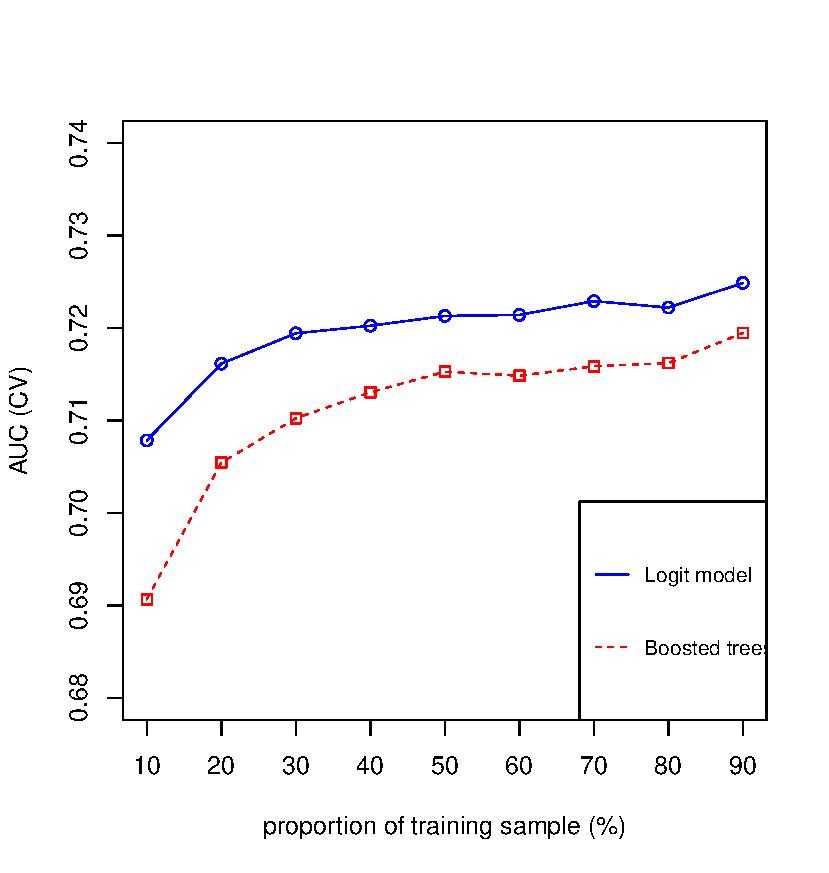
\includegraphics[scale=.6]{Rplot01.pdf}
	\caption{Simple logit model vs boosted trees} 
\end{figure}

\begin{table}[!h]
	\scriptsize
	\caption{Summary of final model fitting}
	\begin{tabular}{l | r r r r}
		\hline
		&Estimate &Std. Error &$Z$ value &$\P(>|Z|)$    \\ \hline
		(Intercept)          &$-$0.0964345  &0.4095179  &$-$0.235 &0.813834    \\
		claim.ind = 1   &0.3547357  &0.0703431   &5.043 &$<0.001$ \\ 
		sales.channel = Online  &0.6104939  &0.1031104   &5.921 &$<0.001$ \\
		sales.channel = Phone   &0.8308277  &0.0628602  &13.217  &$<0.001$\\
		credit = low            &1.5090241  &0.0742303  &20.329  &$<0.001$\\
		credit = medium         &0.6283415  &0.0714722   &8.791  &$<0.001$\\
		zip.code = 2xxxx    &1.3075537  &0.1459212   &8.961  &$<0.001$\\
		zip.code = 5xxxx    &0.3924349  &0.1005980   &3.901 &$<0.001$ \\
		zip.code = 8xxxx    &0.4077199  &0.0949045   &4.296 &$<0.001$ \\
		zip.code = 9xxxx    &0.5112482  &0.1183128   &4.321 &$<0.001$ \\
		n.adults             &$-$0.0154627  &0.0296857  &$-$0.521 &0.602450    \\
		n.children           &0.0145507  &0.0240757   &0.604 &0.545597    \\
		tenure               &0.0378312  &0.0063443   &5.963 &$<0.001$ \\
		len.at.res           &$-$0.0919500  &0.0247059  &$-$3.722 &$<0.001$ \\
		ni.age               &$-$0.0538695  &0.0090701  &$-$5.939 &$<0.001$ \\
		ni.marital.status    &$-$0.4807568  &0.0712064  &$-$6.752 &$<0.001$ \\
		n.adults:n.children  &0.0528847  &0.0093483   &5.657 &$<0.001$ \\
		len.at.res:ni.age    &0.0015699  &0.0005479   &2.865 &0.004169 \\
	\end{tabular}
\end{table}

\section{R codes}

\lstinputlisting[language=R]{rcode.r}








\end{document}

%------------------------------------------------------------------------------
% The End 
%------------------------------------------------------------------------------
